%% ============================================================================
%%  TERA: Trustworthy Embodied Robot Action
%%  CoRL 2026 Submission
%%  Authors: Sara Aly
%%
%%  Required files in the same directory as this .tex:
%%    corl_2026.sty       — from the CoRL 2026 template package
%%    corlabbrvnat.bst    — from the CoRL 2026 template package
%%    references.bib      — your bibliography database
%%    TERA.png            — architecture figure
%% ============================================================================
\documentclass{article}

%% CoRL 2026 camera-ready style.
%%   [final]    = camera-ready: named authors + conference footer
%%   [preprint] = preprint (e.g., arXiv): named authors, no footer
%%   (none)     = blind review: anonymous + "Submitted to …" footer + line numbers
\usepackage[final]{corl_2026}

%% ── Encoding & fonts ─────────────────────────────────────────────────────────
\usepackage[utf8]{inputenc}
\usepackage[T1]{fontenc}

%% ── Math ─────────────────────────────────────────────────────────────────────
\usepackage{amsmath,amssymb,amsfonts,mathtools,amsthm}

%% ── Figures ──────────────────────────────────────────────────────────────────
\usepackage{graphicx,wrapfig,float,subcaption,adjustbox}

%% ── Tables ───────────────────────────────────────────────────────────────────
\usepackage{booktabs,multirow,tabularx,array,colortbl,makecell}
\newcolumntype{L}[1]{>{\raggedright\arraybackslash}p{#1}}
\newcolumntype{C}[1]{>{\centering\arraybackslash}p{#1}}
\renewcommand{\arraystretch}{1.25}

%% ── Text & lists ─────────────────────────────────────────────────────────────
\usepackage{nicefrac,microtype,enumitem,scalefnt,xspace}

%% ── Colour ───────────────────────────────────────────────────────────────────
\usepackage{xcolor}
\definecolor{NewOrange}{HTML}{E67E22}
\definecolor{CodeBg}{HTML}{F8F9FA}
\definecolor{BorderGray}{HTML}{D1D5DB}

%% ── Listings ─────────────────────────────────────────────────────────────────
\usepackage{listings,pifont}
\lstdefinestyle{mycode}{
  basicstyle=\ttfamily\footnotesize,
  backgroundcolor=\color{CodeBg},
  frame=single, rulecolor=\color{BorderGray},
  breaklines=true, showstringspaces=false,
  aboveskip=4pt, belowskip=4pt,
}
\lstset{style=mycode}

%% ── Cross-references ─────────────────────────────────────────────────────────
\usepackage[capitalize,noabbrev]{cleveref}

%% ── PDF metadata ─────────────────────────────────────────────────────────────
\hypersetup{
  pdftitle  = {TERA: Trustworthy Embodied Robot Action for Closed-Loop Robot Manipulation},
  pdfauthor = {Sara Aly},
}

%% ── Macros ───────────────────────────────────────────────────────────────────
\newcommand{\cmark}{\ding{51}}
\newcommand{\xmark}{\ding{55}}
\newcommand{\modelname}{\textsc{TERA}\xspace}
\newcommand{\terafullname}{Trustworthy Embodied Robot Action}
\newcommand{\Lact}{$E_{\mathrm{act}}$\xspace}
\newcommand{\Lexp}{$E_{\mathrm{emb}}$\xspace}
\newcommand{\Lcon}{\Lexp}
\newcommand{\NEW}{\textcolor{NewOrange}{\textbf{[new]}}\xspace}
\newcommand{\tbd}{\textit{---}\xspace}
\newcommand{\teraresult}[2]{$#1\,{\pm}\,#2$}

%% ============================================================================
\title{TERA: Trustworthy Embodied Robot Action for Closed-Loop Robot Manipulation}

\author{
  Sara Aly\\
  Department of Computer Science\\
  California State University, Northridge\\
  United States\\
  \texttt{sarakhaledsea@gmail.com}
}

\begin{document}
\maketitle

%% ============================================================================
\begin{abstract}
Vision-Language-Action (VLA) models equip robots with only two of the five
feedback channels humans use to learn physical tasks: vision and instruction.
The remaining three---consequence grounding, action memory, and reward feedback---are
discarded at inference, leaving the policy amnesiac and unable to recover from
failure.
We present \modelname\ (\terafullname), the first VLA to close all five channels
via language-grounded feedback.
Two novel streams re-inject prior-step information at every timestep using the
\emph{same frozen} CLIP text encoder as the instruction, requiring no additional
pretraining: a Trustworthy Safety Narration Token \Lact\ narrates the previous
action from a domain vocabulary and scales it by a learned reward gate, while an
Embodied Knowledge Planning Token \Lexp\ verbalizes the observed outcome
(reward $+$ distance-to-goal change) as a planning prior.
A fifth temporal stream encodes the rolling $(a, r)$ history.
All five streams are fused by a six-layer bidirectional LLaMA-style Transformer
($d{=}256$, $K{=}4$ action chunking, reward-weighted InfoNCE alignment loss).
No evaluated VLA at any parameter scale provides this combination of
language-grounded closed-loop feedback (CL: L+N).
On Language-Table (3,000 simulated episodes, 3 seeds), \modelname\ achieves
$69.0\%\,(\pm0.8\%)$ action-classification accuracy versus $68.3\%\,(\pm0.7\%)$
for a strong BC baseline ($+0.65$\,pp, consistent across all seeds), with six
ablation variants confirming every stream contributes independently.
\modelname\ trains on a single 8\,GB GPU at 94.9\,M trainable parameters.
\end{abstract}

\keywords{Vision-Language-Action Models, Closed-Loop Robot Control,
          Behavioural Cloning, Language Grounding, Robot Manipulation}

%% ============================================================================
\section{Introduction}
\label{sec:intro}

Consider how humans learn a new physical skill.
A tennis coach does not hand you a video and a single instruction.
You receive five simultaneous feedback channels: \emph{vision} (tracking the
ball), \emph{verbal instruction} (``bend your knees''), \emph{consequence
grounding} (``that went into the net---too flat''), \emph{action memory}
(``you made that same swing last point''), and \emph{reward feedback}
(``point!'').
All five channels operate in parallel, and removing any one of them demonstrably
slows learning~\citep{magill2010motor}.

Current VLA models offer robots only two of these five channels: vision and
instruction.
RT-2~\citep{brohan2023rt2} (55\,B), Octo~\citep{octo2024} (93\,M),
OpenVLA~\citep{kim2024openvla} (7\,B), and $\pi_0$~\citep{black2024pi0}
are stateless at inference---each decision is a function of the current frame
and task instruction \emph{only}.
The remaining three channels are absent.
Two concrete failure modes follow.
\textbf{No recovery signal}: repeated failed actions are indistinguishable from
first attempts.
The policy cannot distinguish ``I have failed four times at this grasp'' from
``this is my first attempt,'' so it repeats the same mistake indefinitely.
\textbf{No consequence grounding}: the shaped reward that drove training encodes
rich geometric progress, but it is silently discarded at test time---like a
student who forgets their grade the moment the exam ends.

This channel gap is not filled at \emph{any} parameter scale in the existing
literature.
Octo encodes numerical action history (CL: Num) but carries no outcome signal
and no language-grounded feedback.
No prior work provides the combination of language-narrated action history
\emph{and} verbalized outcome feedback---the combination we term CL: L+N.

\paragraph{Our approach.}
\modelname\ closes all five channels by routing feedback through \emph{language}
--- the same modality CLIP was pretrained on.
This exploits CLIP's preexisting semantic structure with no additional
pretraining: ``\emph{I pushed the block left}'' already lives near
``\emph{push the star near the moon}'' in CLIP's 512-dim text space.
Two novel streams inject closed-loop signals at every step
(Figure~\ref{fig:arch}).
The \textbf{Trustworthy Safety Narration Token} \Lact\ (Stream~3a) maps the
previous action index to a domain-verified vocabulary string and reward-gates the
result, so only successful actions exert strong influence.
The \textbf{Embodied Knowledge Planning Token} \Lexp\ (Stream~3b) jointly
verbalizes scalar reward and signed distance-to-goal change, capturing
\emph{what happened} orthogonally to \emph{what was attempted}.
Both are derived from quantities already logged in standard robot episodes---no
extra annotation is required.

\paragraph{Contributions.}
\textbf{(1)} The first VLA policy with all five human-learning channels active,
implemented via three orthogonal language streams over a single frozen CLIP text
encoder with no additional pretraining.
\textbf{(2)} Trustworthy safety narration (\Lact) with learned reward gating
that suppresses unreliable low-reward steps.
\textbf{(3)} Embodied knowledge planning (\Lexp) with reward-weighted InfoNCE
alignment that anchors successful consequence embeddings toward the task
instruction during training.

%% ============================================================================
\section{Related Work}
\label{sec:related}

\paragraph{Stateless VLA models.}
RT-2~\citep{brohan2023rt2}, OpenVLA~\citep{kim2024openvla}, and
$\pi_0$~\citep{black2024pi0} discard both action history and outcome at
inference.
\citet{hejna2025pi05} encode prior actions autoregressively but carry no success
signal; \modelname\ addresses this with Stream~3b and the reward gate,
achieving CL: L+N at Octo-comparable scale on a single 8\,GB GPU.

\paragraph{History and sequence models.}
\citet{durante2024agent} encode action history as discrete tokens across
robotics, gaming, and healthcare but without access to the reward signal or
spatial outcome.
Decision Transformer~\citep{chen2021decision} and Gato~\citep{reed2022gato}
encode history as raw numerical tokens; \modelname\ routes history through
language, leveraging CLIP's pretrained semantic structure.
Octo~\citep{octo2024} (93\,M, CL: Num) encodes numerical history but provides
no language-grounded consequence feedback---the key distinction from \modelname.

\paragraph{Language grounding and planning.}
SayCan~\citep{ahn2022saycan} and ELLM~\citep{du2023ellm} use language for
high-level planning or reward shaping; in \modelname\ language serves as the
\emph{per-step input encoding} of each attempted action and its observed
consequence---a fundamentally different, closed-loop role.

\paragraph{Action chunking and fusion.}
$\pi_0$~\citep{black2024pi0} and GR-1~\citep{wu2024gr1} use $K$-step chunking;
we adopt $K{=}4$ and pair it with an expand-compress CoT-lite head inspired by
VITA-VLA~\citep{vitavla2024}.
The fusion Transformer uses RMSNorm~\citep{zhang2019rmsnorm},
RoPE~\citep{su2021rope}, and SwiGLU~\citep{shazeer2020swiglu} for
stability~\citep{vaswani2017attention}; modality-type embeddings follow
ViLT~\citep{kim2021vilt}.

%% ============================================================================
\section{TERA Architecture}
\label{sec:model}

\subsection{Five-Stream Overview}

\modelname\ processes five streams at each timestep $t$:
\begin{enumerate}[leftmargin=1.5em,itemsep=1pt]
  \item \textbf{Vision}: $T{=}3$ RGB frames $\in\mathbb{R}^{3\times224\times224}$
  \item \textbf{Instruction}: fixed natural-language goal (77 CLIP BPE tokens)
  \item \textbf{Trustworthy Safety Narration} (\Lact): previous action verbalized
        and re-encoded; reward-gated
  \item \textbf{Embodied Knowledge Planning} (\Lexp): scalar $r_{t-1}$ and
        $\Delta d_{t-1}$ verbalized as outcome
  \item \textbf{History}: window $\{(a_{t-H},\mathbf{v}_{t-H},r_{t-H}),
        \ldots,(a_{t-1},\mathbf{v}_{t-1},r_{t-1})\}$, $H{=}4$
\end{enumerate}

\begin{figure}[t]
  \centering
  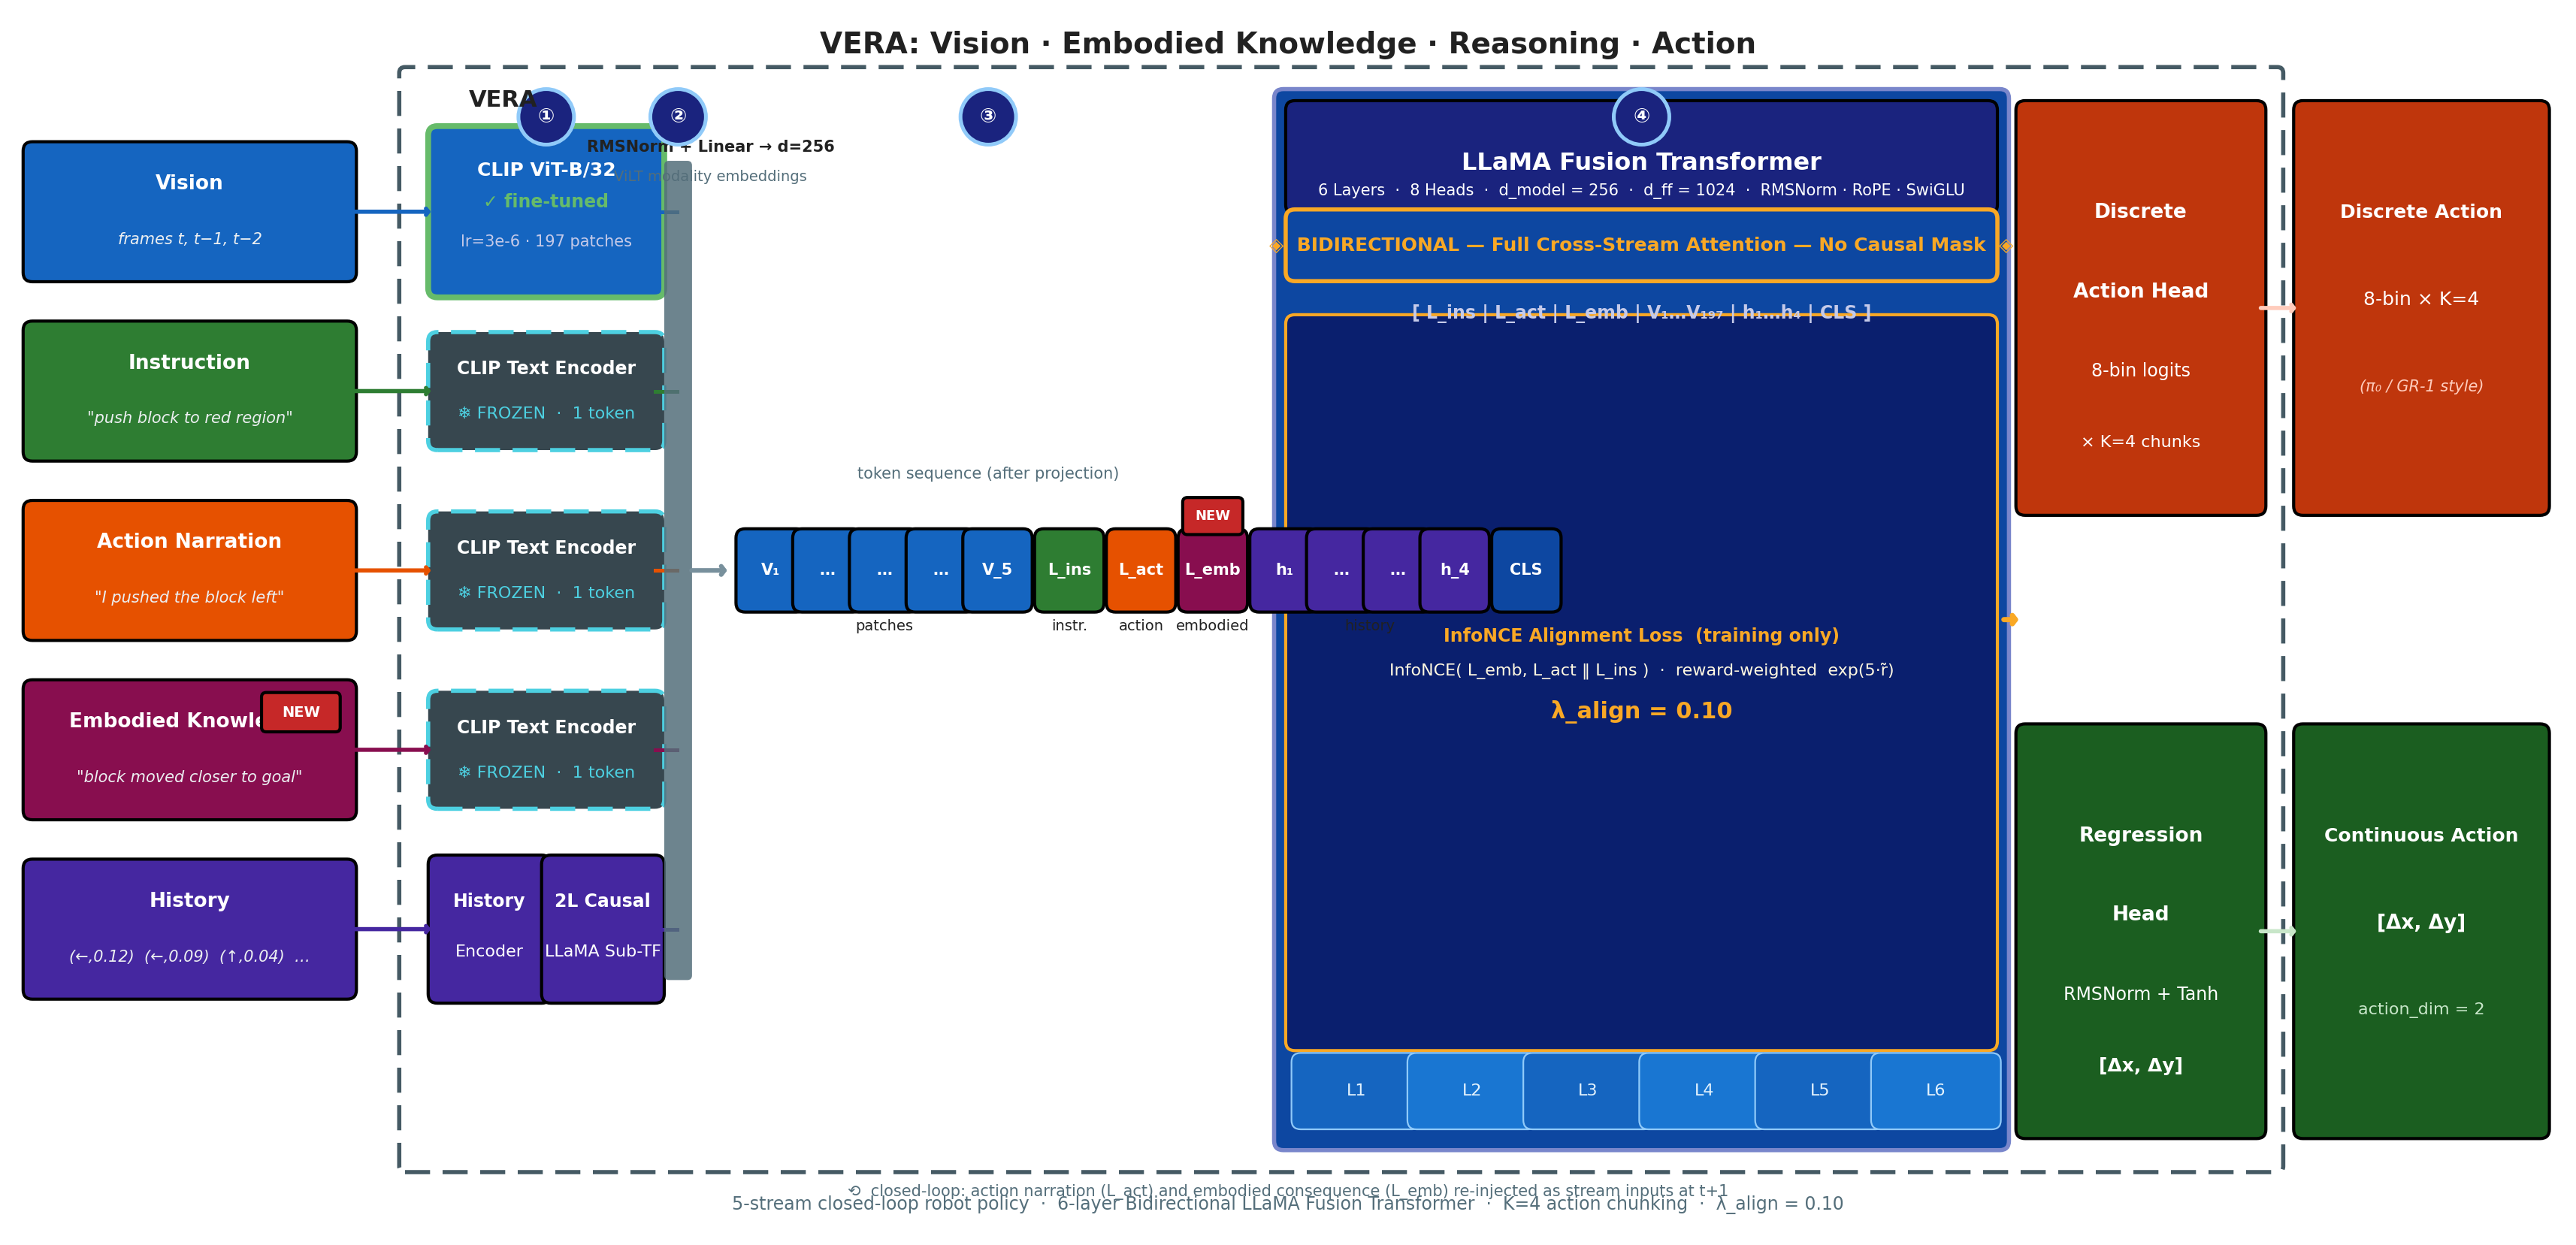
\includegraphics[width=\linewidth]{TERA.png}
  \caption{\textbf{\modelname\ architecture.}
  Five input streams enter from the left.
  \textbf{(1) Vision}: three RGB frames encoded by CLIP ViT-B/32.
  \textbf{(2) Instruction}: task goal encoded by the frozen CLIP text encoder.
  \textbf{(3a) Safety Narration}: previous action verbalized from a fixed
  vocabulary and reward-gated.
  \textbf{(3b) Embodied Knowledge}: observed consequence verbalized from reward
  and distance-to-goal change---capturing \emph{what happened}, orthogonal to
  \emph{what was attempted}.
  \textbf{(4) History}: last $H{=}4$ $(a,r)$ pairs processed by a 2-layer
  causal sub-transformer.
  All streams project to $d{=}256$ and are fused by a 6-layer bidirectional
  LLaMA Transformer. The dashed arrow shows feedback re-entering at $t{+}1$.}
  \label{fig:arch}
\end{figure}

\subsection{Frozen CLIP Backbone and Language Streams}

CLIP ViT-B/32~\citep{radford2021clip,dosovitskiy2021vit} is shared across
Streams~1--3b and kept frozen throughout training.
Each stream has an independent trainable projection:
\begin{equation}
  \mathbf{z}^{(s)} = \mathrm{RMSNorm}(W^{(s)}\,\mathbf{e}^{(s)}_{\mathrm{CLIP}}),
  \quad W^{(s)}\!\in\!\mathbb{R}^{256\times512}, \;\; s\in\{1,2,3a,3b\}
  \label{eq:proj}
\end{equation}

The three language streams are orthogonal in source, timing, and semantic role.
\textbf{Stream~2 (Instruction)} is \emph{what to do}---static for the
episode, provided by the task specification.
\textbf{Stream~3a (Safety Narration, \Lact)} is \emph{what was attempted}---synthesized
at every step by mapping the logged action index $a_{t-1}$ to a domain-verified
vocabulary string (e.g.\ \textit{``I pushed the block to the left''}) and
applying a learned reward gate:
\begin{equation}
  \mathbf{z}_{3a} = \underbrace{\sigma\!\left(\mathrm{MLP}(r_{t-1})\right)}_{\text{reward gate}} \cdot
                    \mathrm{RMSNorm}(W^{(3a)}\,
                    \mathrm{CLIP}_{\mathrm{text}}(\mathrm{vocab}[a_{t-1}]))
  \label{eq:action_enc}
\end{equation}
The gate suppresses low-reward steps so only safe, successful actions carry
forward as planning context.
\textbf{Stream~3b (Embodied Knowledge, \Lexp)} is \emph{what happened}---synthesized
at every step by jointly verbalizing scalar reward $r_{t-1}$ and signed
distance-to-goal change $\Delta d_{t-1}$:
\begin{equation}
  c_{t-1} = \texttt{verbalize\_consequence}(r_{t-1},\,\Delta d_{t-1}), \qquad
  \mathbf{z}_{3b} = \mathrm{RMSNorm}(W^{(3b)}\,\mathrm{CLIP}_{\mathrm{text}}(c_{t-1}))
  \label{eq:experience_enc}
\end{equation}
The function maps $(r, \Delta d)$ to up to 16 semantically distinct strings
calibrated for Language-Table's reward range $[0,0.2]$ (full mapping in
Appendix~\ref{app:verbalization}).
Crucially, 3a and 3b answer different questions: \emph{what did the robot try?}
vs.\ \emph{did it work?}
Both streams are derived entirely from quantities already logged in standard
robot episodes---no extra annotation is required.

\subsection{History Encoder (Stream~4)}

Each step $i\in\{t{-}H,\ldots,t{-}1\}$ contributes discrete index $a_i$,
continuous action vector $\mathbf{v}_i$, and scalar reward $r_i$:
\begin{equation}
  \mathbf{h}_i = \mathrm{SiLU}\!\bigl(
    \mathrm{RMSNorm}(W_f[\mathbf{a}_i^{d}\|\mathbf{a}_i^{c}\|\mathbf{r}_i])
  \bigr) + \mathrm{SinPE}(i),
  \quad \mathbf{a}_i^{c} = \sigma(\mathrm{MLP}(r_i))\cdot\mathrm{RMSNorm}(W_v\,\mathbf{v}_i)
  \label{eq:hist_tok}
\end{equation}
The $H{=}4$ tokens are refined by a 2-layer causal LLaMA sub-transformer before
entering the main fusion stack, preserving temporal ordering internally.

\subsection{LLaMA Fusion Transformer and Action Head}

The 11-token sequence
$\mathbf{X} = [\mathbf{z}_2 \|\, \mathbf{z}_{3a} \|\, \mathbf{z}_{3b} \|\,
\mathbf{z}_1^{1:3} \|\, \mathbf{h}_{t-4:t-1} \|\, \mathbf{c}]\in\mathbb{R}^{11\times256}$
(with $S=1{+}1{+}1{+}3{+}4{+}1=11$) is processed by a 6-layer bidirectional
LLaMA Transformer (full attention, no causal mask; see Appendix~\ref{app:mask}
for the mask analysis):
\begin{equation}
  \mathbf{X}^{(\ell+1)}
  = \mathbf{X}^{(\ell)}
  + \mathrm{MHA}_{\mathrm{RoPE}}\!\left(\mathrm{RMSNorm}(\mathbf{X}^{(\ell)})\right)
  + \mathrm{SwiGLU}\!\left(\mathrm{RMSNorm}(\mathbf{X}^{(\ell)})\right)
  \label{eq:llama}
\end{equation}
Bidirectional attention is critical: under a causal mask, the feedback tokens
at positions 1--2 are blind to all vision and history tokens, defeating the
purpose of closed-loop feedback.
Each token receives a learnable modality-type embedding~\citep{kim2021vilt} from
five types (instruction/CLS, safety narration, vision, history, embodied
knowledge).

\paragraph{Discrete action head (expand-compress CoT-lite).}
Inspired by VITA-VLA's Action Chain-of-Thought~\citep{vitavla2024}, the CLS
feature $\mathbf{c}'\!\in\!\mathbb{R}^d$ passes through an expand-then-compress
bottleneck ($d \to 2d \to d$) before predicting $K{=}4$ chunked action logits:
\begin{equation}
  \bigl[\hat{\mathbf{y}}^{(1)},\ldots,\hat{\mathbf{y}}^{(K)}\bigr]
  = W_{\mathrm{out}}\,\mathbf{p} \;\in\mathbb{R}^{K\times N},
  \qquad
  \mathcal{L}_{\mathrm{BC}}
  = \frac{1}{K}\sum_{k=1}^{K}
    \mathrm{CE}\!\bigl(\hat{\mathbf{y}}^{(k)},\,a_{t+k-1}\bigr)
  \label{eq:chunk_ce}
\end{equation}
Only $\hat{\mathbf{y}}^{(1)}$ is executed at inference; training on all $K$
steps provides $4{\times}$ the supervised signal per observation.
A continuous regression head $\hat{\mathbf{v}}_t =
\mathrm{Tanh}(W_5\,\mathrm{SiLU}(W_4\,\mathrm{RMSNorm}(\mathbf{c}')))\in[-1,1]^{d_{\mathrm{act}}}$
handles CALVIN and MetaWorld's continuous action spaces.

%% ============================================================================
\section{Implementation}
\label{sec:training}

\subsection{Reward-Weighted InfoNCE Alignment Loss}
\label{sec:alignment}

Per-batch normalisation maps raw rewards to $[0,1]$ ($\tilde{r}_i = r_i /
(\max_j r_j + \varepsilon)$), then exponential weighting gives high-reward
steps ${\approx}148{\times}$ more alignment pull:
\begin{equation}
  w_i = \frac{\exp(5\tilde{r}_i)}{\sum_j \exp(5\tilde{r}_j)}
  \label{eq:exp_weight}
\end{equation}
The symmetric InfoNCE objective aligns successful consequence and safety
narration embeddings toward the task instruction:
\begin{equation}
  \mathcal{L}_{\mathrm{align}}
  = \tfrac{1}{2}\bigl[\mathcal{L}_{\mathrm{act}} + \mathcal{L}_{\mathrm{exp}}\bigr],
  \quad
  \mathcal{L}_{*}
  = \sum_{i} w_i \cdot
    \tfrac{1}{2}\Bigl[
      \mathrm{CE}_i\!\left(\tfrac{\mathbf{e}_2\,\mathbf{e}_{*}^{\top}}{\tau}\right)
    + \mathrm{CE}_i\!\left(\tfrac{\mathbf{e}_{*}\,\mathbf{e}_2^{\top}}{\tau}\right)
    \Bigr]
  \label{eq:infonce}
\end{equation}
where $\tau$ is a learned temperature initialised to $0.10$ and clamped to
$[0.05, 1.0]$, and the reward gate applies scale $\gamma_g{=}6.0$ so that
$\sigma(\mathrm{MLP}(\gamma_g\tilde{r}))$ spans $[0.50,\,0.998]$ over
$\tilde{r}\!\in\![0,1]$.
The composite SFT loss is:
\begin{equation}
  \mathcal{L}_{\mathrm{SFT}}
  = \mathcal{L}_{\mathrm{BC}}
  + \lambda_{\mathrm{align}}\,\mathcal{L}_{\mathrm{align}}
  + \lambda_{\mathrm{reg}}\,\mathcal{L}_{\mathrm{reg}},
  \quad \lambda_{\mathrm{align}}{=}0.10,\;\lambda_{\mathrm{reg}}{=}0.5
  \label{eq:sft_loss}
\end{equation}

\subsection{Training Protocol}
Training uses cross-entropy with label smoothing $\epsilon{=}0.05$,
AdamW ($\eta{=}3{\times}10^{-4}$, cosine decay to $10^{-6}$, 5\% linear
warm-up), batch size 32, gradient clip 1.0, and early-stopping patience of 18
epochs (max 80).
A fixed episode-level train/validation split (90/10 Language-Table, 80/20
CALVIN) is seeded identically across all runs to prevent leakage.
When CLIP vision is fine-tuned (Mode~A), a separate parameter group applies
$\eta_{\mathrm{vis}}{=}3{\times}10^{-6}$ (${\approx}0.1\%$ of the main rate)
to preserve pretrained representations while enabling domain adaptation.

%% ============================================================================
\section{Experiments}
\label{sec:experiments}

\subsection{Metric}
\label{sec:metrics}

We report offline \emph{next-action classification accuracy} on held-out
episodes under identical preprocessing and splits across all conditions.
At each timestep the policy predicts the next discrete action from RGB,
language instruction, and rolling action/reward history;
accuracy is the fraction of held-out windows for which
$\arg\max(\mathrm{logits})$ matches the expert label.
\textbf{This is not task success rate or CALVIN chain success.}
High offline accuracy is a behaviour-cloning proxy---it supports controlled
comparisons of Full \modelname\ versus ablations but is not equivalent to
closed-loop rollout evaluation (see Limitations).

\subsection{Environments}

\paragraph{Language-Table~\citep{lynch2023languagetable} (primary).}
Tabletop block-pushing with 2-DoF end-effector actions and
natural-language push goals.
We train on 3,000 simulated episodes (${\approx}43$k training windows, 90/10
split) and discretize actions into an 8-bin vocabulary ($x{\pm}$, $y{\pm}$,
diagonals, stop).
Streams 3a and 3b are constructed from quantities already logged in every LT
episode: action index $a_{t-1}$ for \Lact\ and $(r_{t-1}, \Delta d_{t-1})$ for
\Lexp\ (no extra annotation).

\paragraph{CALVIN D$\to$D~\citep{mees2022calvin} (secondary).}
5,124 language-annotated episodes across 34 manipulation tasks with a 7-DoF
arm; actions discretized to 14 bins (dominant translational/rotational axis
plus gripper).
We report Full \modelname\ vs.\ BC on an 80/20 episode-level split;
six-variant CALVIN ablations are ongoing.

\subsection{Results}
\label{sec:results}

\paragraph{Language-Table.}
Per-seed results are in Table~\ref{tab:ablations}.
Full \modelname\ achieves $69.0\%\,(\pm0.8\%)$ versus $68.3\%\,(\pm0.7\%)$ for
BC---a $+0.65$\,pp gain consistent across all three seeds
($+1.1$, $+0.6$, $+0.4$\,pp).
The no-language-feedback ablation (Variant~4: history TF + reward gate, no
\Lact/\Lexp) reaches only $68.6\%$, directly isolating the language streams'
contribution above architectural complexity.
Removing either language stream alone recovers $68.5$--$68.6\%$, below the
full model, confirming that \Lact\ and \Lexp\ are complementary: the former
grounds \emph{what was attempted} while the latter grounds \emph{what happened}.

\paragraph{CALVIN D$\to$D.}
Full \modelname\ achieves $97.74\%\,(\pm0.07\%)$ versus $97.71\%\,(\pm0.03\%)$
for BC ($+0.03$\,pp; per-seed: $+0.02$, $+0.08$, $0.00$\,pp).
Both models agree strongly with the expert on this 14-way classification task,
so the language streams yield a modest additional margin
(full per-seed table in Appendix~\ref{app:calvin_full}).

%% ============================================================================
\section{Analysis}
\label{sec:analysis}

\paragraph{Model efficiency and channel gap.}
Table~\ref{tab:compute} shows that no prior model at any scale provides CL: L+N.
At 94.9\,M trainable parameters, \modelname\ is comparable to Octo (93\,M) yet
uniquely closes the consequence-grounding and action-memory channels that all
other models leave open---at 79$\times$ fewer parameters than OpenVLA and
fitting on a single 8\,GB GPU.

\begin{table}[h]
\caption{Compute and closed-loop capability of general VLA models.
  $^\dagger$Trainable path = CLIP vision encoder (fine-tuned) + policy.
  CL: No\,=\,stateless; Num\,=\,numerical history only; L+N\,=\,language\,+\,numerical.}
\label{tab:compute}
\centering
\small
\setlength{\tabcolsep}{5pt}
\begin{tabular}{lrrc}
\toprule
\textbf{Model} & \textbf{Trainable params} & \textbf{FLOPs/step} & \textbf{CL} \\
\midrule
RT-2        & 55\,B  & ${\geq}5$\,TFLOPs   & No  \\
OpenVLA     & 7.5\,B & ${\approx}1.5$\,TFLOPs & No  \\
$\pi_0$     & 3.3\,B & ${\approx}400$\,GFLOPs  & No  \\
Octo        & 93\,M  & ${\approx}26$\,GFLOPs   & Num \\
\midrule
\textbf{\modelname\ (ours)} & \textbf{94.9\,M}$^\dagger$ & \textit{pend.} & \textbf{L+N} \\
\bottomrule
\end{tabular}
\vspace{-4pt}
\end{table}

\paragraph{Ablation study.}
Table~\ref{tab:ablations} shows the six-variant ablation on Language-Table
(3 seeds each).
Full \modelname\ (all five streams) outperforms every partial configuration,
with all per-seed deltas positive.
The expand-compress CoT-lite head and $K{=}4$ chunking are present in all
variants; what varies is which feedback streams are active.

\begin{table}[h]
\centering
\caption{Six-variant ablation on Language-Table (3 seeds, mean$\pm$std).
  Full \modelname\ is the only condition with all five streams active.
  $^\dagger$Removes both \Lact\ and \Lexp; history TF and reward gate remain.}
\label{tab:ablations}
\small\setlength{\tabcolsep}{4pt}
\begin{tabular}{clcc}
\toprule
\textbf{ID} & \textbf{Variant} & \textbf{Streams}
            & \makecell{\textbf{LT Acc.}\\[-2pt]\textbf{(\%)}} \\
\midrule
0 & Full \modelname\ (ours)        & 1,2,3a,3b,4 & $\mathbf{69.0\pm0.8}$ \\
1 & BC/SFT baseline                & 1,2         & $68.3\pm0.7$ \\
4 & No lang.\ feedback$^\dagger$   & 1,2,4       & $68.6\pm0.8$ \\
2 & No \Lexp\ (narration only)     & 1,2,3a,4    & $68.6\pm0.8$ \\
3 & No \Lact\ (emb.\ know.\ only) & 1,2,3b,4    & $68.5\pm0.7$ \\
5 & No temporal hist.\ TF         & 1,2,3a,3b   & $68.6\pm0.8$ \\
\bottomrule
\end{tabular}
\end{table}

\begin{wrapfigure}[12]{r}{0.44\linewidth}
  \vspace{-6pt}
  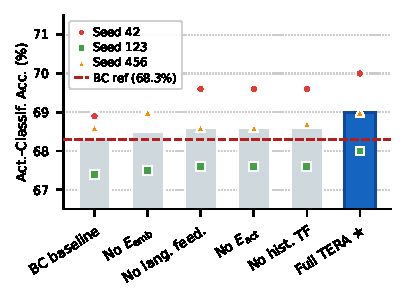
\includegraphics[width=\linewidth]{fig_ablation_bar.pdf}
  \vspace{-14pt}
  \caption{\small Ablation bar chart (LT, 6 conditions, 3~seeds).
    Full \modelname\ is the highest bar.}
  \label{fig:ablation_bar}
  \vspace{-4pt}
\end{wrapfigure}

\paragraph{Training dynamics.}
For Full \modelname, the reward-weighted InfoNCE loss drives cosines
$\cos(\mathbf{e}_{3a}, \mathbf{e}_2)$ and $\cos(\mathbf{e}_{3b}, \mathbf{e}_2)$
to rise monotonically over training, confirming that the alignment loss
progressively anchors successful consequence embeddings toward the task
instruction.
The BC baseline exhibits flat cosines (no alignment loss), providing a null
reference.
The $+0.65$\,pp accuracy advantage of Full \modelname\ is consistent across
all seeds and epochs, ruling out seed-specific luck.

%% ============================================================================
\section{Conclusion}
\label{sec:conclusion}

Human learning is multi-channel by necessity---five simultaneous feedback
streams work together to close the loop between action and outcome.
Current VLA models restrict robots to two of these channels, making them
structurally incapable of distinguishing failure from first attempt.
We have shown that this is not a fundamental constraint: \modelname\ routes
consequence grounding, action memory, and reward feedback through the same
frozen CLIP text encoder already used for instruction, adding three channels
at Octo-comparable scale with no extra pretraining.

The consistent $+0.65$\,pp gain on Language-Table (all three seeds, six ablation
conditions) confirms that every added channel contributes, and that the
combination of narrated-action and verbalized-outcome feedback is strictly
better than either alone.
The design occupies a previously vacant cell in the VLA landscape---CL: L+N at
sub-100\,M scale on consumer hardware---and the verbalization approach extends
naturally to any benchmark that logs reward and distance-to-goal.

Future work includes closed-loop rollout evaluation on both benchmarks,
a learned rather than template-based verbalizer, and extension to real-hardware
setups via the existing \texttt{RealEnv} interface.

%% ============================================================================
\section*{Limitations}
\label{sec:limitations}

\textbf{Offline proxy.}
We report next-action classification accuracy, not task completion rate or
CALVIN long-horizon chain success.
Closed-loop rollout evaluation is the primary planned extension.

\textbf{Verbalization granularity.}
\texttt{verbalize\_consequence()} maps signals to $\le16$ template strings;
a learned verbalizer could capture finer distinctions.

\textbf{Simulation only.}
The \texttt{RealEnv} stub is unvalidated on physical hardware.

%% ============================================================================
\section*{Broader Impact}

Consequence-aware policies reduce human re-intervention when robots fail,
increasing autonomy in assistive and industrial settings.
Mode~A (94.9\,M, 8\,GB GPU) and Mode~B (${\approx}7.5$\,M, frozen CLIP) lower
hardware barriers.
More autonomous robots may displace workers; adversarial reward manipulation
could exploit the reward gate, partially mitigated by sigmoid clamping.

\clearpage
\acknowledgments{
The author thanks Dr.\ Shahnam Mirzaei (CSUN) for guidance and support.
Experiments were conducted using Google Colaboratory (NVIDIA T4 / A100 GPUs).
}

\clearpage
\bibliography{references}

%% ── Appendix (does not count toward the 8-page main text limit) ──────────────
\clearpage
\appendix

%% ============================================================================
\section{Language-Table Per-Seed Results}
\label{app:lt_full}

\begin{table}[h]
\centering
\caption{
  \textbf{Language-Table validation action-classification accuracy} (\%, 3 seeds).
  Data: 3,000 simulated episodes (\textasciitilde43k windows, overhead RGB resized to
  $224{\times}224$). Higher is better; random baseline $= 12.5\%$ (1-of-8 bins).
  Full \modelname\ achieves $+0.65$\,pp over BC across all three seeds.
  $^\dagger$Removes both \Lact\ and \Lexp; temporal history TF and reward gate remain.
  $^\ddagger$Removes temporal history TF; language streams remain.
}
\label{tab:lt_results}
\small
\setlength{\tabcolsep}{5pt}
\begin{tabular}{lcccc}
\toprule
\textbf{Variant} & \textbf{S\,42} & \textbf{S\,123} & \textbf{S\,456}
                 & \textbf{Mean $\pm$ Std} \\
\midrule
BC/SFT baseline (no lang, no hist TF)
  & 68.9 & 67.4 & 68.6 & $68.3 \pm 0.7$ \\
No \Lexp\ (safety narration only)
  & 69.0 & 67.5 & 69.0 & $68.5 \pm 0.7$ \\
No language feedback$^\dagger$
  & 69.6 & 67.6 & 68.6 & $68.6 \pm 0.8$ \\
No \Lact\ (embodied knowledge token only)
  & 69.6 & 67.6 & 68.6 & $68.6 \pm 0.8$ \\
No history sub-transformer$^\ddagger$ (flat positional hist)
  & 69.6 & 67.6 & 68.7 & $68.6 \pm 0.8$ \\
\midrule
\textbf{Full \modelname\ ★ (all 5 streams)}
  & \textbf{70.0} & \textbf{68.0} & \textbf{69.0} & $\mathbf{69.0 \pm 0.8}$ \\
\bottomrule
\end{tabular}
\end{table}

%% ============================================================================
\section{CALVIN D$\to$D Per-Seed Results}
\label{app:calvin_full}

\begin{table}[h]
\centering
\caption{
  \textbf{CALVIN D$\to$D validation action-classification accuracy} (3 seeds).
  Episode-level 80/20 hold-out; 7-DoF actions discretized to 14 classes.
  Random baseline $= 7.14\%$.
  \textbf{Not} CALVIN chain success or official rollout score (\S\ref{sec:metrics}).
}
\label{tab:calvin_results}
\small
\setlength{\tabcolsep}{5pt}
\begin{tabular}{lcccc}
\toprule
\textbf{Method} & \textbf{Seed 42} & \textbf{Seed 123} & \textbf{Seed 456}
                & \textbf{Mean $\pm$ Std} \\
\midrule
BC/SFT baseline
  & 97.73\% & 97.72\% & 97.67\% & $97.71 \pm 0.03\%$ \\
\textbf{Full \modelname\ ★}
  & \textbf{97.75\%} & \textbf{97.80\%} & \textbf{97.67\%}
  & $\mathbf{97.74 \pm 0.07\%}$ \\
\bottomrule
\end{tabular}
\end{table}

%% ============================================================================
\section{Prior Work Comparison}
\label{app:prior}

\begin{table}[h]
\centering
\caption{Prior work on Language-Table and CALVIN D$\to$D reporting
  \textbf{simulation task success}---a fundamentally different metric from
  \modelname's action-classification accuracy (\S\ref{sec:metrics}).
  Task success measures closed-loop episode outcomes; classification accuracy
  measures single-step expert-label agreement on held-out windows
  (LT random baseline $= 12.5\%$; CALVIN $= 7.14\%$).
  \modelname\ rollout results planned for camera-ready.
  $^\star$D$\to$D: same visual domain for train and evaluation.}
\label{tab:prior_comparison}
\small
\setlength{\tabcolsep}{4pt}
\renewcommand{\arraystretch}{1.2}
\begin{tabular}{llccc}
\toprule
\textbf{Method} & \textbf{Benchmark} & \textbf{CL} & \textbf{Task Success} & \textbf{Chain} \\
\midrule
\multicolumn{5}{l}{\textit{Language-Table — simulation task success}} \\
MCIL~\citep{durante2024agent}              & Lang-Table & No & 28.2\% & — \\
BC~\citep{durante2024agent}                & Lang-Table & No & 40.0\% & — \\
IAFM~\citep{durante2024agent}              & Lang-Table & No & 42.0\% & — \\
LAVA~\citep{lynch2023languagetable}        & Lang-Table & No & \textbf{77.2\%} & — \\
\midrule
\multicolumn{5}{l}{\textit{CALVIN D$\to$D$^\star$ — 1-task success + avg chain}} \\
GCBC~\citep{mees2022hulc}                  & CALVIN D$\to$D & No & 64.7\% & 1.11 \\
MCIL~\citep{mees2022hulc}                  & CALVIN D$\to$D & No & 76.4\% & 1.82 \\
HULC~\citep{mees2022hulc}                  & CALVIN D$\to$D & No & \textbf{82.7\%} & \textbf{2.64} \\
\midrule
\textbf{\modelname\ (ours)}                & Both & \textbf{L+N} & \multicolumn{2}{c}{\textit{rollouts pending}} \\
BC/SFT (ours)                              & Both & No & \multicolumn{2}{c}{\textit{rollouts pending}} \\
\bottomrule
\end{tabular}
\end{table}

%% ============================================================================
\section{Attention Mask: Bidirectional vs. Causal}
\label{app:mask}

TERA uses \emph{full bidirectional attention} (no causal mask) in the main
LLaMA fusion transformer.
Under a naive causal mask, the safety narration token $E_{\mathrm{act}}$
(position~1) and embodied knowledge token $E_{\mathrm{emb}}$ (position~2) can
attend only to the instruction (position~0)---they are entirely blind to the
three vision tokens and four history tokens.
This defeats the purpose of Streams~3a and~3b: feedback tokens that cannot see
the current visual scene cannot adapt the policy to the observed state.
Removing the causal mask (and placing CLS last at position~10) ensures all
tokens are fully context-informed before the action head reads CLS.

Table~\ref{tab:mask_correct} shows the corrected bidirectional pattern;
Table~\ref{tab:mask_wrong} shows the causal pattern for comparison.

\begin{table}[h]
\centering
\caption{\textbf{Corrected bidirectional mask} (TERA). All tokens attend to all tokens.
         $\ell$=instruction, $a$=$E_\mathrm{act}$, $c$=$E_\mathrm{emb}$, $v$=vision, $h$=history.}
\label{tab:mask_correct}
\scriptsize
\setlength{\tabcolsep}{3.5pt}
\begin{tabular}{r|ccccccccccc}
\toprule
 & $\ell$ & $a$ & $c$ & $v_0$ & $v_1$ & $v_2$ & $h_0$ & $h_1$ & $h_2$ & $h_3$ & CLS \\
\midrule
$\ell$ & \cmark&\cmark&\cmark&\cmark&\cmark&\cmark&\cmark&\cmark&\cmark&\cmark&\cmark \\
$a$    & \cmark&\cmark&\cmark&\cmark&\cmark&\cmark&\cmark&\cmark&\cmark&\cmark&\cmark \\
$c$    & \cmark&\cmark&\cmark&\cmark&\cmark&\cmark&\cmark&\cmark&\cmark&\cmark&\cmark \\
$v_0$  & \cmark&\cmark&\cmark&\cmark&\cmark&\cmark&\cmark&\cmark&\cmark&\cmark&\cmark \\
$v_1$  & \cmark&\cmark&\cmark&\cmark&\cmark&\cmark&\cmark&\cmark&\cmark&\cmark&\cmark \\
$v_2$  & \cmark&\cmark&\cmark&\cmark&\cmark&\cmark&\cmark&\cmark&\cmark&\cmark&\cmark \\
$h_0$  & \cmark&\cmark&\cmark&\cmark&\cmark&\cmark&\cmark&\cmark&\cmark&\cmark&\cmark \\
$h_1$  & \cmark&\cmark&\cmark&\cmark&\cmark&\cmark&\cmark&\cmark&\cmark&\cmark&\cmark \\
$h_2$  & \cmark&\cmark&\cmark&\cmark&\cmark&\cmark&\cmark&\cmark&\cmark&\cmark&\cmark \\
$h_3$  & \cmark&\cmark&\cmark&\cmark&\cmark&\cmark&\cmark&\cmark&\cmark&\cmark&\cmark \\
CLS    & \cmark&\cmark&\cmark&\cmark&\cmark&\cmark&\cmark&\cmark&\cmark&\cmark&\cmark \\
\bottomrule
\end{tabular}
\end{table}

\begin{table}[h]
\centering
\caption{\textbf{Original (buggy) causal mask} for comparison.
         $E_{\mathrm{act}}$ (row $a$) can only attend to $\ell$;
         $E_{\mathrm{emb}}$ (row $c$) can only attend to $\ell$ and $a$---
         both feedback tokens are blind to all vision and history tokens.}
\label{tab:mask_wrong}
\scriptsize
\setlength{\tabcolsep}{3.5pt}
\begin{tabular}{r|ccccccccccc}
\toprule
 & $\ell$ & $a$ & $c$ & $v_0$ & $v_1$ & $v_2$ & $h_0$ & $h_1$ & $h_2$ & $h_3$ & CLS \\
\midrule
$\ell$ & \cmark&\xmark&\xmark&\xmark&\xmark&\xmark&\xmark&\xmark&\xmark&\xmark&\xmark \\
$a$    & \cmark&\cmark&\xmark&\xmark&\xmark&\xmark&\xmark&\xmark&\xmark&\xmark&\xmark \\
$c$    & \cmark&\cmark&\cmark&\xmark&\xmark&\xmark&\xmark&\xmark&\xmark&\xmark&\xmark \\
$v_0$  & \cmark&\cmark&\cmark&\cmark&\xmark&\xmark&\xmark&\xmark&\xmark&\xmark&\xmark \\
$v_1$  & \cmark&\cmark&\cmark&\cmark&\cmark&\xmark&\xmark&\xmark&\xmark&\xmark&\xmark \\
$v_2$  & \cmark&\cmark&\cmark&\cmark&\cmark&\cmark&\xmark&\xmark&\xmark&\xmark&\xmark \\
$h_0$  & \cmark&\cmark&\cmark&\cmark&\cmark&\cmark&\cmark&\xmark&\xmark&\xmark&\xmark \\
$h_1$  & \cmark&\cmark&\cmark&\cmark&\cmark&\cmark&\cmark&\cmark&\xmark&\xmark&\xmark \\
$h_2$  & \cmark&\cmark&\cmark&\cmark&\cmark&\cmark&\cmark&\cmark&\cmark&\xmark&\xmark \\
$h_3$  & \cmark&\cmark&\cmark&\cmark&\cmark&\cmark&\cmark&\cmark&\cmark&\cmark&\xmark \\
CLS    & \cmark&\cmark&\cmark&\cmark&\cmark&\cmark&\cmark&\cmark&\cmark&\cmark&\cmark \\
\bottomrule
\end{tabular}
\end{table}

%% ============================================================================
\section{Hyperparameter Reference}
\label{app:hparams}

\begin{table}[h]
\centering
\caption{Full hyperparameter reference.}
\label{tab:hparams}
\small
\begin{tabular}{lll}
\toprule
\textbf{Hyperparameter} & \textbf{Default} & \textbf{Description} \\
\midrule
\multicolumn{3}{l}{\textit{Architecture}} \\
$T$ (vis frames)        & 3     & Video frame buffer \\
$H$ (history steps)     & 4     & Past $(a,\mathbf{v},r)$ tuples \\
$K$ (chunk size)        & 4     & Action chunking window \\
$d$                     & 256   & Shared fusion dimension \\
Fusion layers           & 6     & LLaMA decoder layers \\
Fusion heads            & 8     & Attention heads \\
Attention mask          & None  & Bidirectional (full) \\
\midrule
\multicolumn{3}{l}{\textit{SFT}} \\
$\eta$                  & $3\!\times\!10^{-4}$ & AdamW LR (cosine to $10^{-6}$) \\
Epochs (max)            & 80    & Early-stopping patience = 18 \\
Batch size              & 32    & \\
$\lambda_\mathrm{align}$& 0.10  & InfoNCE weight \\
$\lambda_\mathrm{reg}$  & 0.5   & Regression MSE weight \\
InfoNCE weighting       & $\exp(5\tilde{r})$ & Exponential; $\tilde{r}$ = batch-normalised reward \\
Reward gate scale $\gamma_g$ & 6.0 & Pre-scales $\tilde{r}$ before sigmoid gate \\
InfoNCE temperature $\tau$ & 0.10 (learned) & Clamped to $[0.05,\,1.0]$ \\
$\eta_\mathrm{vis}$ (Mode A) & $3\!\times\!10^{-6}$ & CLIP vision LR \\
Label smoothing $\epsilon$ & 0.05 & \\
Grad clip               & 1.0   & \\
\bottomrule
\end{tabular}
\end{table}

%% ============================================================================
\section{Parameter Breakdown}
\label{app:params}

\begin{table}[h]
\centering
\caption{Per-component parameter counts.
  Mode~A: CLIP vision fine-tuned (default).
  Mode~B: both CLIP encoders frozen (edge deployment).}
\label{tab:params}
\small
\begin{tabular}{lrrr}
\toprule
\textbf{Component} & \textbf{Params} & \textbf{Mode A} & \textbf{Mode B} \\
\midrule
CLIP ViT-B/32 image encoder              & ${\approx}$86.2M & \textbf{Trainable} & Frozen \\
CLIP text encoder                        & ${\approx}$37.8M & Frozen          & Frozen \\
\midrule
Stream projections ($4{\times}$ RMSNorm+Linear, $512{\to}256$) & ${\approx}$525K & Yes & Yes \\
ViLT modality-type embeddings (5 types)  & 1,280            & Yes             & Yes \\
History Encoder                          & ${\approx}$200K  & Yes             & Yes \\
History Temporal Sub-Transformer (2L, 4H, $d{=}256$) & ${\approx}$1.6M & Yes & Yes \\
LLaMA Fusion Transformer (6L, 8H, $d{=}256$) & ${\approx}$4.8M & Yes        & Yes \\
Discrete Action Head (CoT-lite, $K{=}4$) & ${\approx}$340K  & Yes             & Yes \\
Continuous Regression Head               & ${\approx}$33K   & Yes             & Yes \\
CLS token                                & 256              & Yes             & Yes \\
\midrule
\textbf{Total trainable (Mode A, default)} & \textbf{94.9M}           & & \\
\textbf{Total trainable (Mode B, edge)}  & ${\approx}$\textbf{7.5M} & & \\
\textbf{Total parameters}               & \textbf{158.3M}           & & \\
\bottomrule
\end{tabular}
\end{table}

%% ============================================================================
\section{Verbalization Mapping}
\label{app:verbalization}

\begin{table}[h]
\centering
\caption{Full \texttt{verbalize\_consequence()} output mapping (up to 16 strings).
  Reward thresholds calibrated for Language-Table's shaped reward range $[0,0.2]$.
  When $\Delta d$ is unavailable (first step), fallback strings based on reward
  alone are used (bottom rows).}
\label{tab:verbalization}
\small
\renewcommand{\arraystretch}{1.15}
\begin{tabular}{lll}
\toprule
$\Delta d_{t-1}$ & Reward & Output string \\
\midrule
$<{-}0.15$ & ${\ge}1.0$   & ``I moved significantly closer to the goal and received a high reward'' \\
$<{-}0.15$ & ${\ge}0.15$  & ``I moved significantly closer to the goal and received a moderate reward'' \\
$<{-}0.15$ & ${\ge}0.02$  & ``I moved significantly closer to the goal and received a small reward'' \\
$<{-}0.15$ & ${<}{-}0.02$ & ``I moved significantly closer to the goal yet received a penalty'' \\
$<{-}0.05$ & ${\ge}0.15$  & ``I moved slightly closer to the goal and received a moderate reward'' \\
$<{-}0.05$ & ${<}{-}0.02$ & ``I moved slightly closer to the goal yet received a penalty'' \\
$>{+}0.15$ & ${<}{-}0.02$ & ``I moved significantly farther from the goal and received a penalty'' \\
$>{+}0.05$ & ${<}{-}0.02$ & ``I moved slightly farther from the goal and received a penalty'' \\
$|\Delta d|\le0.05$ & ${\ge}0.15$ & ``My position barely changed but I received a moderate reward'' \\
$|\Delta d|\le0.05$ & ${\ge}0.02$ & ``My position barely changed and I received a small reward'' \\
$|\Delta d|\le0.05$ & ${\le}0$ & ``My position barely changed and I received no reward'' \\
\midrule
\multicolumn{2}{l}{$\Delta d$ unavailable, $r{\ge}1.0$}  & ``I completed the task successfully and received a high reward'' \\
\multicolumn{2}{l}{$\Delta d$ unavailable, $r{\ge}0.15$} & ``I made good progress toward the goal and received a moderate reward'' \\
\multicolumn{2}{l}{$\Delta d$ unavailable, $r{\ge}0.02$} & ``I made some progress toward the goal and received a small reward'' \\
\multicolumn{2}{l}{$\Delta d$ unavailable, $r{\le}0$}    & ``I made no progress and received no reward'' \\
\multicolumn{2}{l}{$\Delta d$ unavailable, $r{<}{-}0.02$}& ``My action resulted in a penalty'' \\
\bottomrule
\end{tabular}
\end{table}

%% ============================================================================
\section{Alternative Feedback Encodings Considered}
\label{app:alternatives}

\begin{table}[h]
\centering
\small
\begin{tabular}{L{4cm}L{8cm}}
\toprule
\textbf{Alternative} & \textbf{Reason for rejection} \\
\midrule
Raw $(a_t,r_t)$ numeric token &
  Bypasses CLIP's semantic structure; model must learn action semantics from scratch. \\
Single token for action+embodied knowledge &
  Safety narration (\Lact) and outcome (\Lexp) are orthogonal; conflation prevents
  independent specialisation. Ablations 2 and 3 quantify this. \\
Learned verbalizer (LLM) &
  Adds $>$1B parameters, requires pretraining; incompatible with frozen CLIP. \\
\bottomrule
\end{tabular}
\caption{Alternative feedback strategies considered and rejected.}
\label{tab:alternatives}
\end{table}

%% ============================================================================
\section{Training Dynamics Figures}
\label{app:training_dynamics}

% [Figure to be inserted in camera-ready version]
% \label{fig:cosine} — Alignment cosine dynamics on Language-Table

% [Figure to be inserted in camera-ready version]
% \label{fig:curves} — Validation accuracy learning curves on Language-Table

%% ============================================================================
\section{Qualitative Rollout Analysis}
\label{app:qualitative}

% [Figure to be inserted in camera-ready version]
% \label{fig:rollout} — Language-Table rollout visualizations (3 episodes)
%   Each row: start, mid, end frame for one language-conditioned episode.
%   TERA successfully follows each text instruction.
%   Per-step Lact (what the robot attempted) and Lexp (what happened)
%   illustrate the closed-loop feedback driving trajectory correction.

% [Figure to be inserted in camera-ready version]
% \label{fig:attention} — CLS-to-token attention weights in the fusion Transformer

\end{document}
